\chapter{Literature Review} \label{LR}

\lhead{Chapter 2. \emph{Literature Review}}
In this section, we will present multiple topics that have been studied to make the implementation choices.

The first sections will be dedicated to a general presentation of some machine learning model that has been considered for this project.

Then we will discuss the current state of the research about imperfect game solving. Presenting the different approaches to this problem.

\section{Machine learning models}
\subsection{Decision Tree}
Decision trees are a way of representing multiple choices and their outcome. As suggested by its name it uses a tree. The root node represents the initial state. Each link represents a decision, and the linked node is the outcome of this decision, usually represented by a new state.

This data structure is particularly useful to represent games. For example, a chess game can be represented by a decision tree where links are moved played and nodes the resulting game state. 

However, one major drawback of this data structure is that it can quickly become complex if there is an important depth (consecutive decision). For instance, for chess, it is impossible to represent a full decision tree because it contains too many different states. A common technique to overcome this limitation is to set a fixed depth and update the decision tree when it is traversed.

Metadata is often added to the link and the nodes to be processed easier by algorithms.

When decision trees are applied to games, an important notion is the Nash equilibrium \citep{nash1950equilibrium}. It represents the optimum decision to take for every state given the fact that the opponent is playing the best response. When a Nash Equilibrium is found for game, it is said that the game is solved. Given the actual computer limitation, such equilibrium can not be computed (or even stored) for complex games. In this case, algorithms try to approximate it, we will discuss it in more detail in section \ref{section:imperfect-game-solving:descision-tree}.

\subsection{Recurrent Neural Network} \label{LR:RNN}
Recurrent Neural Network (RNN) is a type of neural network that uses a part of its output for a part or all its input.

It is particularly interesting for his capacity to have an internal memory and remember the past input. A simple RNN is said to have a short memory and has been used for use-cases involving sequential data.

\subsubsection{LSTM} \label{LR:LSTM}
Long Short-Term Memory (LSTM) is a type of RNN that has increased the popularity of RNN by providing a long memory layout to the existing RNN. It has a specific design that allows having a way better space representation of the input and has proven to works well in many domains. In addition, it is also worth mentioning that it is by design opportune for creativity because it uses its output as input. For example, one project has been made to generate Game Of Throne book \citep{zackthoutt2017}. Or also generating music \citep{kotecha2018generating}.

Given its design, RNN can process and train on a large input given that it is a suitable input for RNN. Where other neural network architectures would not be able to works with it efficiently.

\subsection{Reinforcement Learning} \label{LR:reinforcement-learning}
\subsubsection{Overview}
Reinforcement Learning is a method used to train an algorithm based on experiences. An agent evolves in an environment, makes action, and learns from his mistake.

The basic idea is to have a reward given for an action or a set of actions. While learning the agent will try different actions and the reward will be used to update the algorithm. The update rules are specific to the algorithm used. It is common to use an extra formula to take into consideration the future expected reward.

While learning when the agent needs to take action, there is a set of methods that are common to all algorithms. It either \textbf{exploit}, take the best action (not necessarily optimal yet), or \textbf{explore}, pick a random action. A well-known method is epsilon greedy, it chooses to exploit or explore given predefined probability.

\subsubsection{Q-learning}

Q-learning \citep{watkins1992q} is a popular reinforcement learning method. It learns the Q-values, which are the expected reward of the actions given a state. The formula of a Q-value is: \(Q^{*}(s,a) = \max_{\pi}\sum \left [ r_{t} + yr_{t + 1} + y^{2}r_{t + 2} + ...|s_{t}=s,a_{t}=a, \pi \right ]\). Where \(a\) the the action, \(s\) is the state, \(\pi\) the policy and \(y\) the discount which represent how much the future reward should be take in consideration.

This formula has been limited to small state space due to its learning complexity. Recently research has been done to learn these Q-values with a large state space using neural network, it is Deep Q Network (DQN) \citep{mnih2015human}. This method uses another formula to compute the Q-values, making neural networks way more efficient to train. This method has proven to be successful, it has been used to makes an agent learn how to play 2600 Atari games using only the screen pixels for input \citep{bellemare2013arcade}.

DQN are only using the current state to take action, so it performs poorly when it requires the agent to remember the previous states. Research has been done to overcome this limitation combining DQN with Recurrent Neural Network (DRQN \citep{sorokin2015deep} \cite{chen2016deep}. Both of these methods use an attention system. \citep{chen2016deep} use an attention layer that takes all the previous state of the RNN and selects which information to take (figure \ref{fig:drqn-1}). On the other hand \citep{sorokin2015deep} use a part of the output of their RNN to define the next region of attention (figure \ref{fig:drqn-2}). On the figures you would notice that it is built with a CNN before, it is because these NN were designed to learn how to play Atari games from the screen pixels.

\begin{figure}[ht]
    \centering
    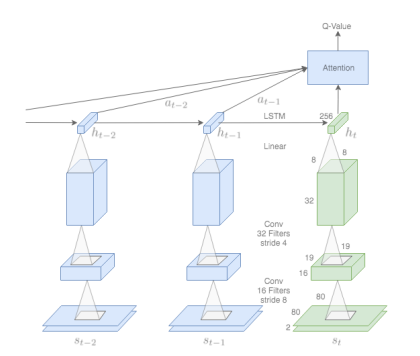
\includegraphics[width=0.7\textwidth]{Figures/drqn-1.png}
    \caption{DRQN with attention layer \citep{sorokin2015deep}}
    \label{fig:drqn-1}
\end{figure}

\begin{figure}[ht]
    \centering
    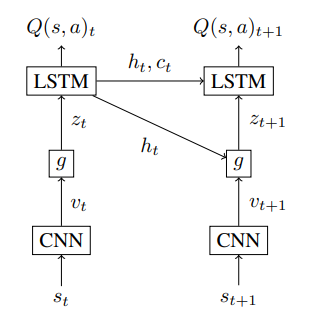
\includegraphics[width=0.5\textwidth]{Figures/drqn-2.png}
    \caption{DRQN with attention \citep{sorokin2015deep}}
    \label{fig:drqn-2}
\end{figure}

\subsection{Evolutionary Algorithms}
% TODO it could use a bit more in the evolutionary and co-evolutionary sections. For instance, a bit more intro to EAs, and maybe some discussion of any related problems co-evolution has been applied to (e.g. designing agents within particular environments, if you can find something like this)

\subsubsection{Overview}
Evolutionary algorithms are a wide category of AI. The idea is inspired by evolutionary biology and natural selection.

The main idea is to have multiple agents (population) evolving together. Each agent represents a potential solution. Agents are evaluated thanks to a fitness function, it defines how well an agent performed. They are evaluated, ranked, a new population is created then a selection is applied to the old generation. This process repeats until a solution is found.

There are multiple methods to perform the selection once the fitness has been calculated. The most commons are:
\begin{itemize}
    \item \textbf{Roulette Wheel Selection} (also called Fitness Proportionate Selection): the probability of selecting an individual is \(\frac{f_{i}}{\sum{f_{k}}} \). It can be represented as a wheel being spin to select the individual. \citep{golberg1989genetic}
    \item \textbf{Tournament Selection}: randomly take individuals from the population, take the best one of them \citep{goldberg1991comparative}
    \item \textbf{Ranked based Selection}: The fitness of the individuals is modified to their rank. For example, the worst individual gets a fitness of one, and the best individual a fitness equal to the population size. Then a roulette wheel selection is done with this new fitness. \citep{goldberg1991comparative}
\end{itemize}
In addition, all these methods have parameters that allow them to either apply more selective pressure or encourage diversity.

To create a new population, multiple methods can be used some may be specific to an EA category. First, an agent will inherit from one individual, all the data from an agent will be copied. From there you can apply mutation, randomly modifying a part of the data. The new agent can also inherit from multiple agents. In this case, there is a crossover/recombination, this mechanic is specific to the implementation of the EA. For example, a simple idea to inherit from two agents would be to take half of the data from one and half of the data from the other one. In addition, crossovers create a lot of diversity. However, if crossovers are made without much consideration it can lead to poor results, this is why there are often rules to guide the crossover.

Co-evolution is a notion we will rely on for this project. Co-evolution learning defines a way of calculating the fitness. It calculates the fitness based on the interaction between the individuals. So, the fitness is subjective and depends on the population. It is particularly useful the cases where a single fixed fitness function is difficult to establish. This differs from traditional EA.

\subsubsection{Collaborative co-evolution}

Collaborative co-evolution consists of evolving multiple agents working together to find a solution, each agent is a part of the solution.

Collaborative co-evolution has been studied for evolving neural network. One research worked on symbiotic adaptive neuro-evolution (SANE) system \citep{moriarty1997forming}. Instead of having each agent representing a neural network, neurons evolve together by being mixed up at every iteration (figure: \ref{fig:sane}). In addition, some neurons form symbiotic relationship, it means that they will likely be matched together in the same layout for the next generation.

\begin{figure}[ht]
    \centering
    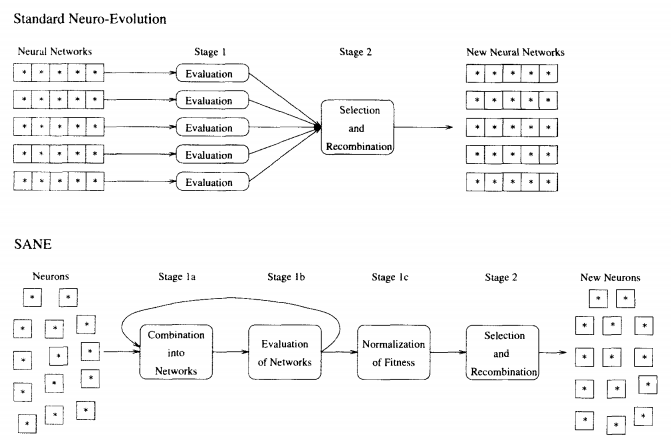
\includegraphics[width=0.85\textwidth]{Figures/sane.png}
    \caption{SANE method compared to Standard Neuro-Evolution \citep{moriarty1997forming}}
    \label{fig:sane}
\end{figure}

This co-evolution method helps to keep a high diversity and claim to have better performance and adaptation than standar elite/tournament method.

I think that such an algorithm is hard to setup, it requires a fine-tuning of the relations between neurons and how you create neural network with them. In addition, in nowadays development environment, such a method can lack performances compared to more supported algorithms.

\subsubsection{Competitive co-evolution} \label{LR:competitive-co-evolution}
Competitive co-evolution consists of multiple agents fighting together to have a higher reward. The fitness is directly based on the competition among the individuals.

One of the major problems of this technique is that it can quickly converge or and get stuck on a sub-optimal solution. In fact, if an agent happens to be stronger than the others then it will ultimately converge to it, even if it is a weak solution \citep{rosin1997new}. To reduce this effect, methods should be used to ensure diversity within the population and speed up the convergence to a perfect solution.

Teaching tests is a method that consists of injecting agents that have a fixed strategy. Those would help distinguish an optimal agent from a sub-optimal agent dominating the population \citep{rosin1997new}.

It is important to keep track of the previous agents, it would ensure that the algorithm is not making cycles and that future agents defeat the previous generation \citep{rosin1997new}. This can be done by injecting agents into the teaching set while training.

Fitness sharing is a method to promote diversity within the population. It is defined to take into account similarity between individuals and lower the fitness given the number of similarities. An idea is to consider each agent as a source of reward and that the reward needs to be shared among all individuals that defeat it. The fitness assigned to an agent is defined by \(\sum_{j \epsilon X}{\frac{1}{N_{j}}}\) where \(N_{j}\) is the number of agents defeating agent \(j\) and \(X\) is the population set \citep{rosin1997new}. Given this method, if a promising agent emerges and defeats an agent that only a few ones can defeat, it will likely be kept in the future generation. In addition, it reduces the convergence to a sub-optimal solution that exploits only a part of the population because the fitness will be divided.

\section{Imperfect game solving} \label{LR:section:imperfect-game-solving}
% TODO say that equilibrium finding if the main area of researsh
\subsection{Overview}
Imperfect game solving is an active field of research, this is a challenging topic for AI. It requires to deal with a high number of possibilities, this encourages to push the scalability limits of some AI models. In addition, it has to deal with unknown information. Furthermore, the evaluation process is tricky, there is no universal way to judge if one action is good or not. Usually, the evaluation is done by playing against other agents/individuals.

Imperfect game solving knowledge is not only about games. It is a way to use AI to works with unknown information. Real-world use cases often deal with unknown information, for example, finance, negotiation, strategic pricing, etc.

One of the most studied game in imperfect game solving is poker. This game has multiple advantages:
\begin{itemize}
    \item It has multiple variants from simple ones such as Kuhn poker to complex ones such as texas hold'em no limits.
    \item It has a wide community with a lot of professional players. This is an important point because the evaluation process may involve playing against professionals players with money, which makes the game results non-biased.
    \item Strategy matters, player choices have an important impact. A good agent playing poker against a weaker opponent will have a high chance to win.
    \item It is a complex game. Bluffing is an important part of the game and is a complex notion.
\end{itemize}

In the following section, we will discuss two main models used in imperfect game solving, Decision Tree and Neural Network. Then we will introduce the notion of exploitability.

\subsection{Decision Tree}
\label{section:imperfect-game-solving:descision-tree}
In imperfect game solving decision trees are widely use and most of the existing approaches use it.

Decision trees are tricky to build for imperfect games because to compute the outcome of a decision it requires to take into account all the possible hidden states.

Ultimately the Nash Equilibrium strategy does not care about hidden state because there is no information about it. An optimum action is given a known state. However, during the equilibrium solving or estimation, the hidden state must be used to estimate/calculate the reward.

For a medium/large game state, abstractions are made to limit the number of representations. For example, in poker, similar combinations of cards are grouped \citep{johanson2013evaluating}.

Successfully poker bot such as Libratus \citep{brown2018superhuman} or Baby Tartanian \citep{brown2016baby} estimates equilibrium on a large game state using MCCFR (Monte Carlo Counterfactual Regret Minimization). It is a reinforcement learning method consisting of playing against itself and updating the strategy based on how much the AI regrets not have selected an action in the past. This process is pre-computed for the first stages, then due to the complexity, it needs to be run in real-time.

Decision tree with equilibrium finding is nowadays the way that has proven to works the best for imperfect game solving.

\subsection{Neural Network}
Neural network has been used for imperfect game solving. We will present two use cases, one using supervised learning and the other one reinforcement learning.

One of the most successful uses of Neural Network in imperfect game solving is DeepStack \citep{moravvcik2017deepstack}, a poker bot. It uses neural network to approximate the opponent's counterfactual values and so decide which action to take (figure \ref{fig:deepstack}). One neural network is trained for each stage of the game, each one uses the output of the previous neural network as input. They trained these neural networks using supervised learning from randomly generated poker situations.

\begin{figure}[ht]
    \centering
    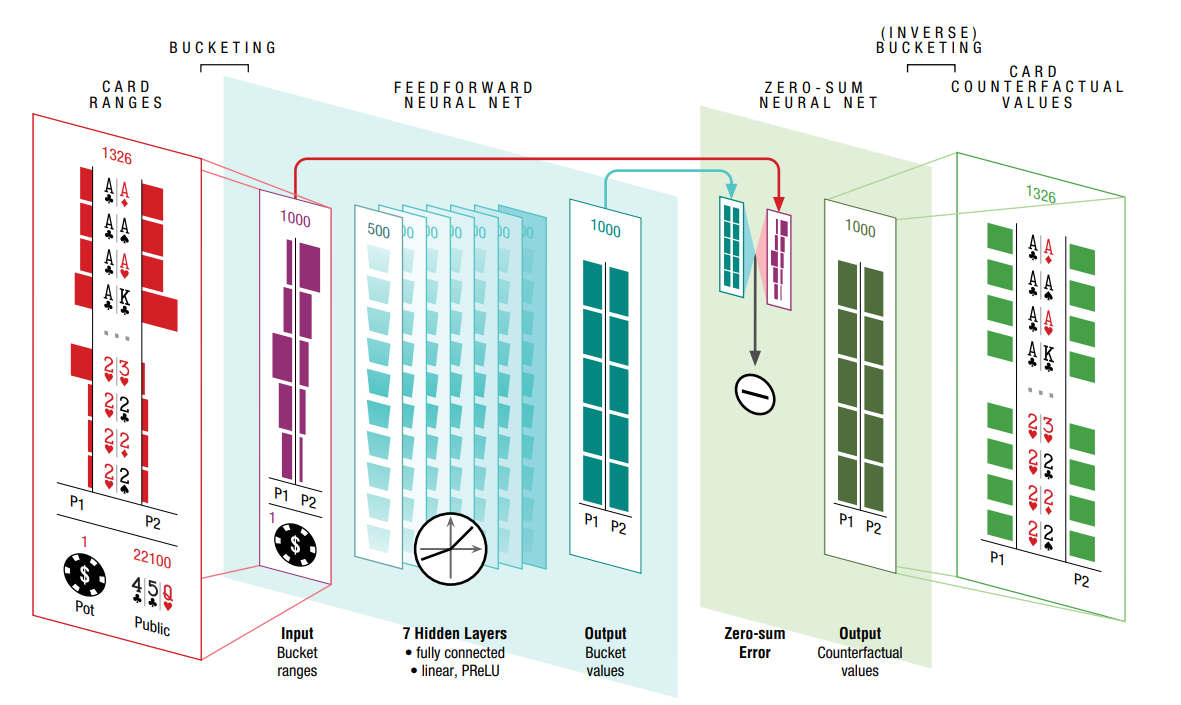
\includegraphics[width=1\textwidth]{Figures/deepstack.png}
    \caption{DeepStack counterfactual value network \citep{moravvcik2017deepstack}}
    \label{fig:deepstack}
\end{figure}

Rlcard \citep{zha2019rlcard} is an implementation of Deep-Q learning \citep{DBLP:journals/corr/MnihKSGAWR13} for imperfect game solving. It also uses NSFP (Neural Fictitious Self-Play) to manage the learning environment and DeepCFR to train the agent. The neural network is always fed with the same "info set" which is an absolute representation of the game. The idea is to bind an action to an info set thanks to neural network. It has proved that neural network and reinforcement learning can perform well in this area. In addition, this implementation is not specific to a game and can be applied to any imperfect game. On the other hand, due to this not specific implementation, it can not have abstraction. So, games with a large game state such as poker texas hold'em are not expected to have good performance.

\subsection{Exploitation in imperfect game solving}
Exploitation aims to identify and exploit the weaknesses of an opponent. Opponent modelling is the process of identifying the way the opponent is playing. If an opponent model is accurate exploiting it is straightforward.

Exploitation is a tricky process because it comes with exploitability. While deviating from the optimum to maximize the reward based on the previous action of the opponent there is a chance to be exploited. This is known as the "get taught and exploited problem" \citep{SANDHOLM2007382}.

It is called safe opponent exploitation when exploitation is done without possibility of being exploited and unsafe opponent exploitation when the possibility of being exploited is assumed.

\subsubsection{Unsafe opponent exploitation}
One research has been done on modelling the opponent in large information games \citep{ganzfried2011game}. They decided to assume that by exploiting an opponent they were going to be exposed to exploitation. They used an algorithm called Deviation-Based Best Response (DBBR), which statistically learns the deviation made by an opponent from an approximated equilibrium. In this way, it can exploit the statistical mistake made by an opponent.

One interesting thing about this research is that it relies on concepts available in every game, which is Nash-equilibrium and best response. This means that their method can be generalized to other imperfect games.

On the other hand, this algorithm has major issues, it requires to play a high number of games against an opponent to have a relatively good model. Even with that, the model will only be accurate in the early stages because it will not have enough sample of the opponent strategy in the middle/late. Indeed, decision trees are immense for imperfect games and it is unrealistic to have a usable model opponent for all the stages of the game with this algorithm.

The exploitation is also purely statistical, it can not model complex behavior. It also treats all the games with the same weight, it does not take an account the temporally of each game. For example, it would be impossible to model anger, the fact that if an opponent loses the previous game it will play aggressively the next one.

\subsubsection{Safe opponent exploitation}
Safe opponent exploitation is the idea of exploiting an opponent without the capacity of being exploited. It was stated that it was not possible \citep{ganzfried2011game}.

However, a recent research on safe opponent exploitation has proven that it was possible on some game \citep{ganzfried2015safe}. They introduce the notion of gift, profitable strategies that can be used by identifying sub-optimal opponent behavior. These gifts are defined formally for each game and can not be generalized.

Safe opponent exploitation relies heavily on equilibrium and plays the equilibrium strategy most of the time. During the evaluation process of this study, they played against dump agents, that for example always fold. It is hard to estimate how important does safe exploitation would make a difference with a more subtle sub-optimal agent.

The main issue with safe exploitation is that the extra reward from exploiting the opponent is limited by an important set of rules. In addition, the safe exploitation is game-specific and is impossible to generalize, it needs to be re-proven for each use case.

% TODO say somewhere that the game state size if equal to the info and action set size (or something like that)
